\section*{Week 41}
\subsection*{What Happend This Week}
This week we have started brainstorming on the \ac{GUI} for the app, and made
some considerations as to what will be shown. On \autoref{fig:sketch} a sketch
is shown for our \ac{GUI}, currently the idea is to show where the person is
located on the policitcal spectrum based on its twitter profile. We have also
considered showing where the person stand compared to the users friends. Aside
from that we made some smaller edits to the report.

\begin{figure}[H] 
	\centering 
	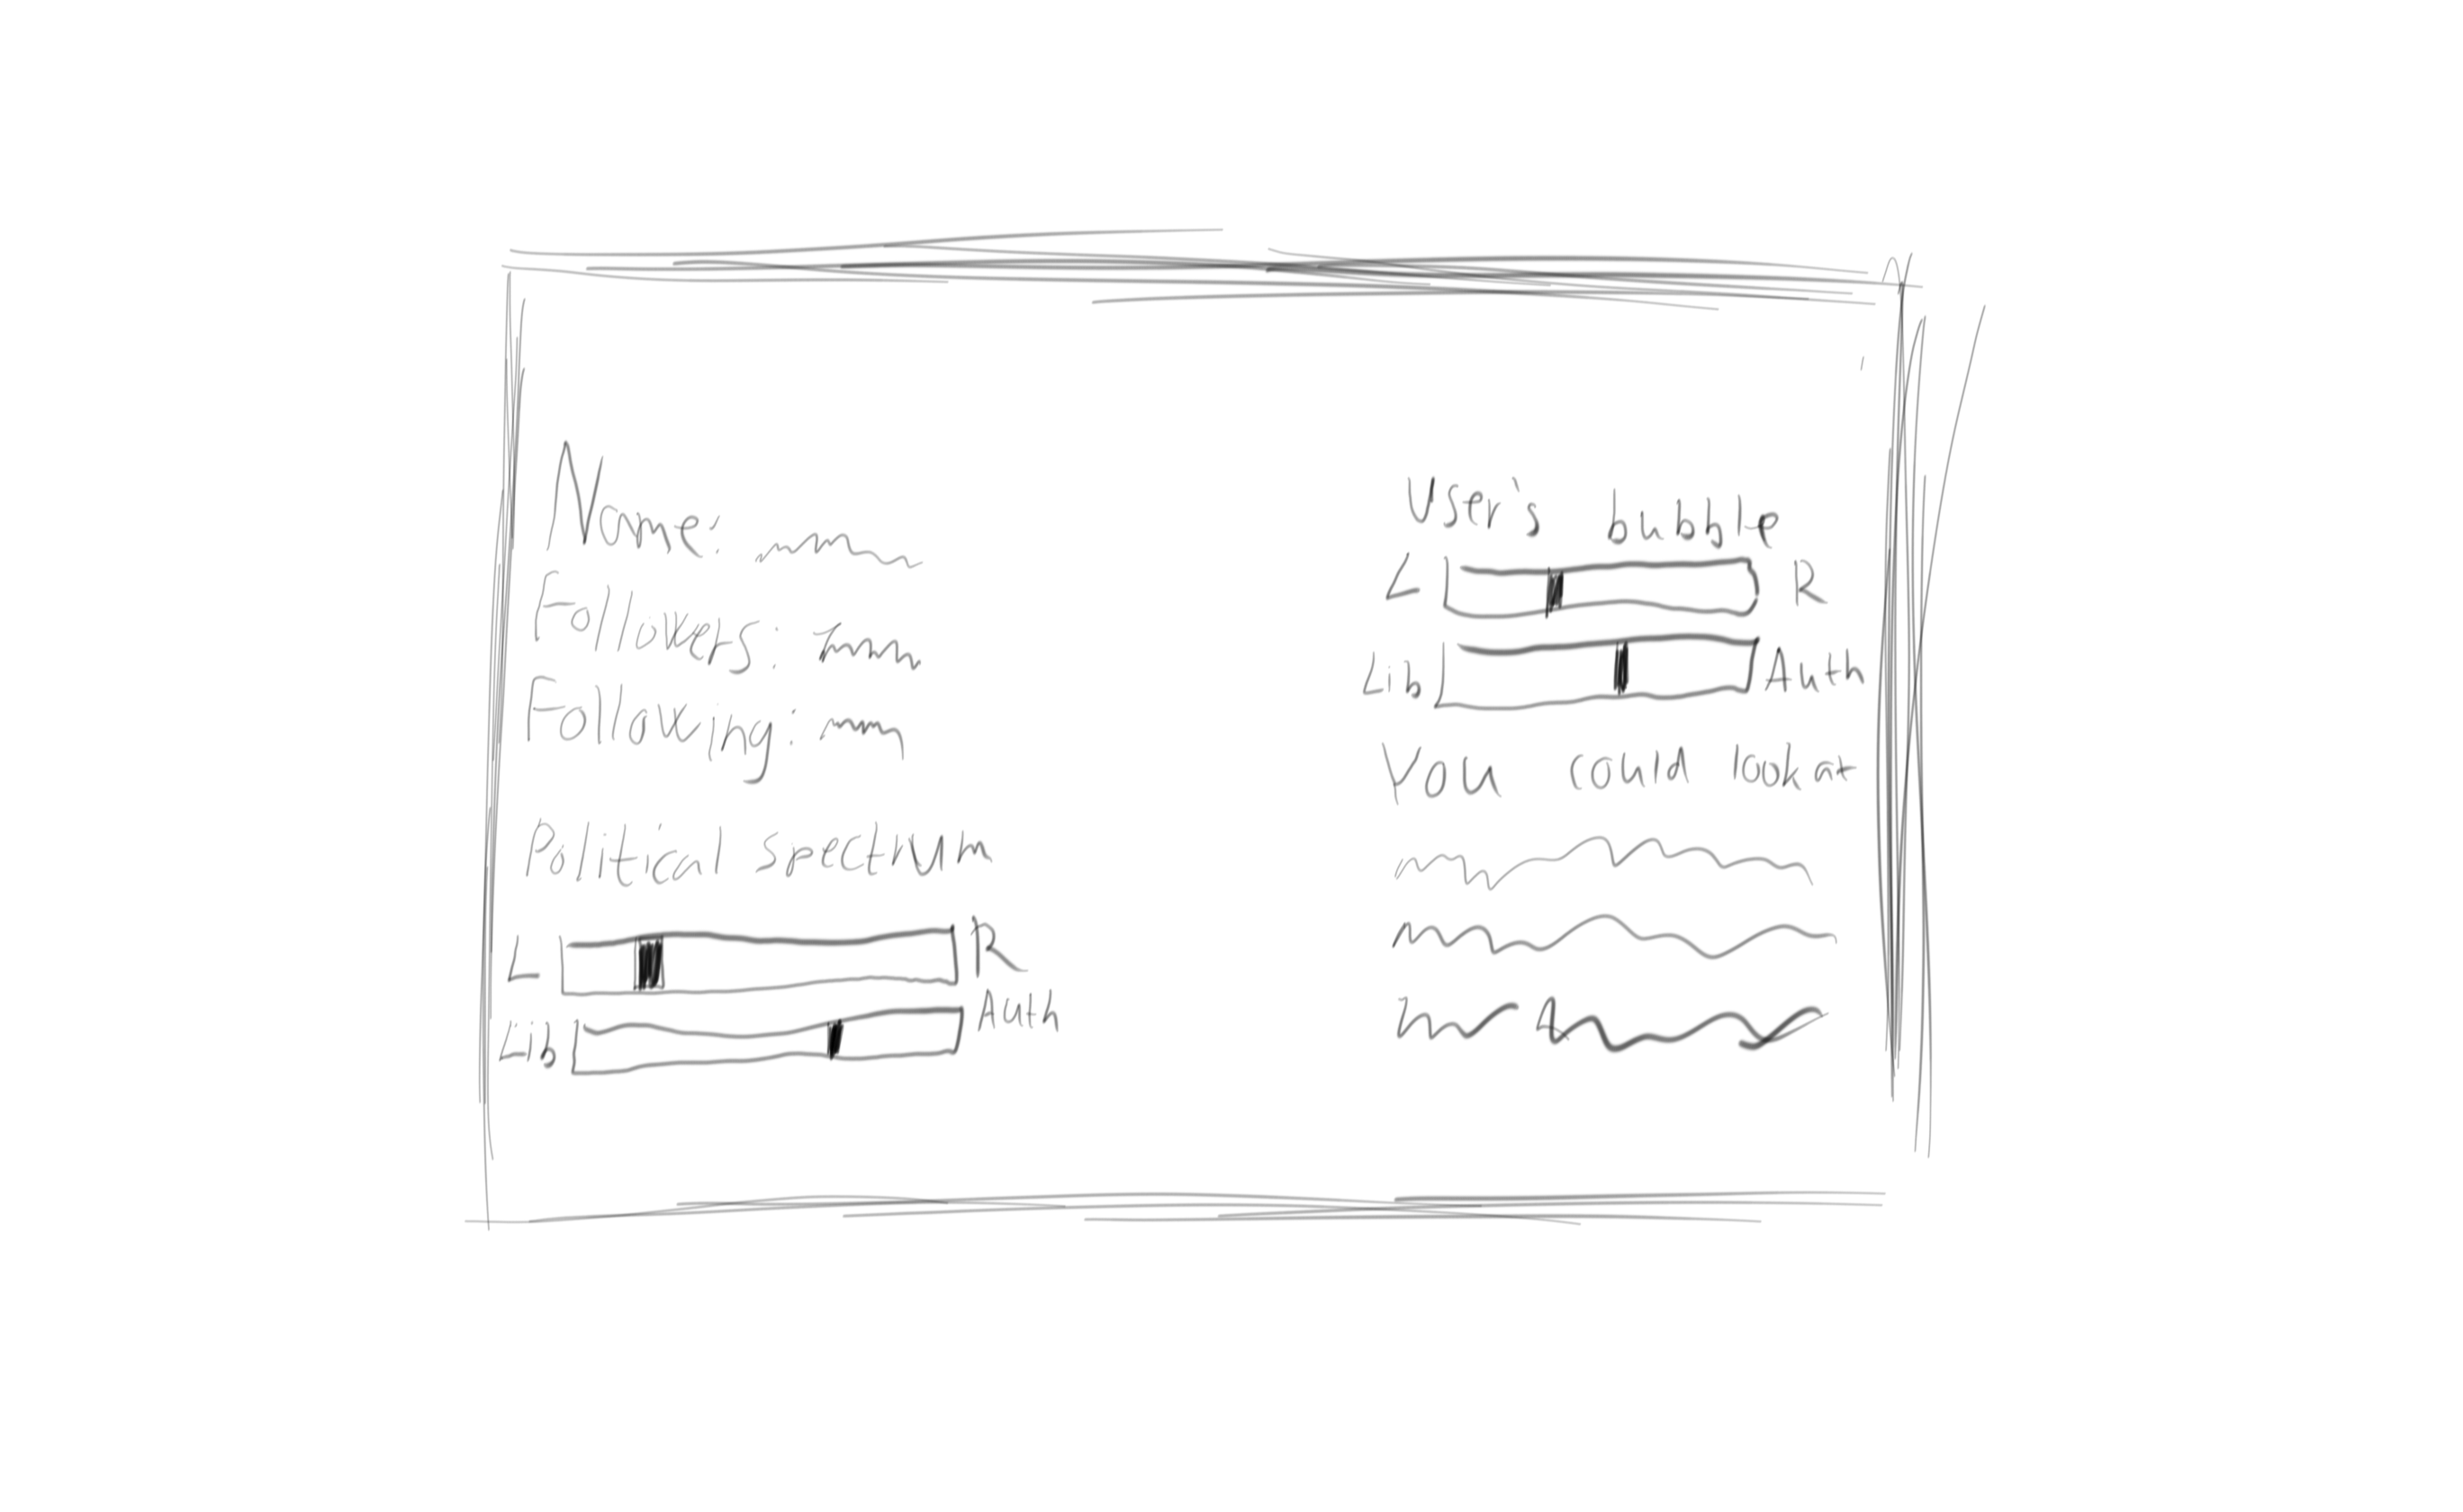
\includegraphics[width = 0.7\textwidth]{figures/guisketch2.png}
	\caption{A sketch of our initial idea for a \ac{GUI}}.
	\label{fig:sketch}
\end{figure}]

\subsection*{Evaluation}
During the development of the \ac{GUI} we found that we had not given much
thought to what we wanted to preset the viewer with, and while designing it came
up with other cool features we could estrapulate from it. It might have been
usefull to do this a little earlier, although it would probably not have
changed much.
We were also told by our suporvisor that we did not need to bring much from
courses and ideas were fitting, our research chappter needed to be restructured
a little to be more coherent.


\subsection*{Next Week}
We will finish the restructuring of the report and continiue development on the
program, and get started on developing the front end.



% Worked on a GUI section (DEB terms), specifically we drew a storyboard and a
% sketch of the gui.
% 
% Reworked text and fixed grammatical errors. Reworked the title in analysis,
% began on problem statement, and finished working on most of the analysis.
% 
% Fixed the threads of the program We are now able to find the average political
% value of a bias.
% 
% Scheme delivery